The first Persian stance detection dataset (\cite{stance_persian})  is used in this project. \cite{stance_persian} dataset can be used in stance detection, summarization, and fake news detection tasks. This dataset contains 2124 news articles that cover information about 534 claims. Number of samples in each class is specified in table \ref{tbl:sdatapie}. Claims are retrieved from Shayeaat \footnote{shayeaat.ir} and Fakenews\footnote{fakenews.ir} websites. Each sample contains 3 different labels for the stance detection task, containing the article's headline toward the claim, the article's body toward the claim, and the article's headline toward its body. Samples are tagged manually. Four following classes are considered for stance classifying:
\begin{itemize}
	\item {\color{green!70!black}\textbf{Agree:}} The article clearly states that the claim is True without any ambiguity or amphibology. 
	\item {\color{red!70!black}\textbf{Disagree:}} The article clearly refutes that the claim without any ambiguity or amphibology. 
	\item {\color{yellow!70!black}\textbf{Discuss:}} The article contains information about the claim but doesn't have any evaluation of its truth. 
	\item {\color{gray!}\textbf{Unrelated:}} There isn't any information about the claim in the article.
\end{itemize}
Dataset samples distribution in each class is illustrated in Figure \ref{fig:datacom}. According to Figure \ref{fig:datacom}, the ratio of \textit{Agree}. Besides, \textit{Disagree} labels are much lower than the others and there is a potential risk for models to be biased on \textit{Unrelated} and \textit{Discuss}. Also, the percentage of \textit{Unrelated} label is higher in headline to claim than article to claim. A headline can be considered as a summary of news body. So, unlike news text, news headline may not have enough information to evaluate a claim.  Moreover, ratio of \textit{Discuss} to \textit{Agree} and \textit{Disagree} is higher in Article to claim in comparison to headline to claim. Accordingly, it seems that news agencies choose more controversial headlines to appeal reader's attention.

Furthermore, this dataset covers each claim veracity according to related news articles. Veracity labels statistics (FakeNews Dataset) is illustrated in table \ref{tbl:fakedata}. In this dataset, the main focus has been on published fake news, this can be inferred from figure \ref{fig:fake}. Three following labels are also considered for classifying news veracity for each claim-headline and claim-body pairs.

\begin{itemize} 
	\item {\color{green!70!black}\textbf{True:}} Reliable news agencies have asserted that this claim is a fact.
	\item {\color{red!70!black}\textbf{False:}} Unreliable news agencies have spread data about this claim and reliable news agencies have considered this claim as hearsay.
\item {\color{gray}\textbf{Unknown:}} There isn't enough integrity between reliable news agencies sources.
\end{itemize}




\begin{table}
	\centering
	\caption{Samples distribution in four classes of Persian stance dataset.}
	\setlength{\extrarowheight}{5pt}
	\begin{tabularx}{1\textwidth} { 
			| >{\centering\arraybackslash}X 
			| >{\centering\arraybackslash}X 
			| >{\centering\arraybackslash}X 
			| >{\centering\arraybackslash}X 
			| >{\centering\arraybackslash}X | }
		\hline
		Label & Agree & Disagree & Unrelated & Discuss \\
		\hline \hline
		Headline to claim & 628  & 210  & 932 & 824  \\
		\hline
		Article to claim & 189  & 374  & 797 & 1196  \\
		\hline
		
	\end{tabularx} 
	\label{tbl:sdatapie}
\end{table}

\begin{figure}%
	\centering
	\subfloat[\centering Artcile to Claim]{{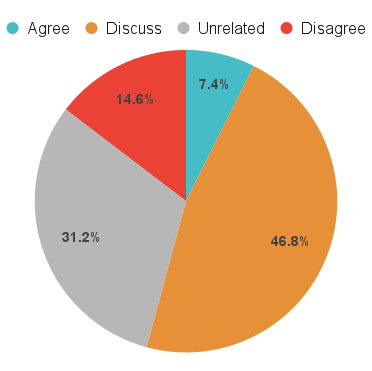
\includegraphics[width=6cm]{statistics/stance/a2c.png} }}%
	\qquad
	\subfloat[\centering Headline to claim ]{{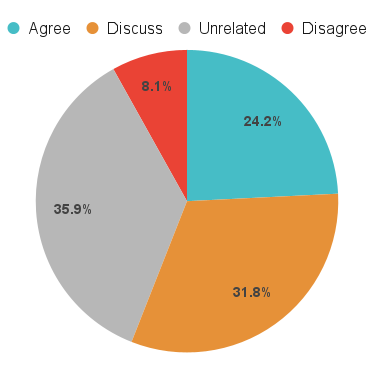
\includegraphics[width=6cm]{statistics/stance/h2c.png} }}%
	\caption{Comparison between article-to-claim and headline-to-claim labels, samples distribution in \cite{stance_persian} dataset.}%
	\label{fig:datacom}%
\end{figure}

\begin{table}
	\centering
	\caption{Fake news data set statistics}\label{fake-news-dataset}
	\small
	\setlength{\extrarowheight}{5pt}%
	\begin{tabularx} {0.7\textwidth}{ 
			| >{\centering\arraybackslash}X 
			| >{\centering\arraybackslash}X 
			| >{\centering\arraybackslash}X 
			| >{\centering\arraybackslash}X | }
		\hline 
		{\bf Used case}      & {\bf True} & {\bf False} & {\bf Unknown} \\ \hline  \hline
		{Test set}     &      {20}      &      {250}      &  {8} \\ 
		\hline
		{Training set}    &     {91}      &      {1003}       &   {35}\\
		\hline
			{Overall}    &     {111}      &      {1253}       &   {43}\\
		\hline
	\end{tabularx}
	\label{tbl:fakedata}
\end{table}

\begin{figure}%
	\centering
	{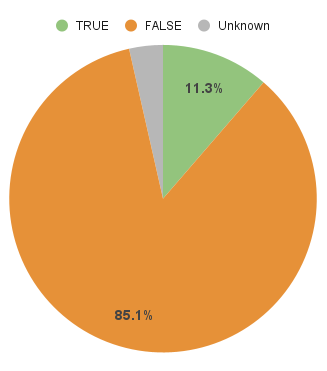
\includegraphics[width=5.5cm]{statistics/stance/fake.png} }
	\caption{Claim veracity label's distribution in \cite{stance_persian} dataset.}%
	\label{fig:fake}%
\end{figure}
  
